% Provenance (never printed): see sources/outline_sources.md (Year 1:
% observational astronomy, photometry). Telescopes, angular resolution,
% gratings, the Doppler effect and the black-body laws are owned by the
% physics series and recalled here. Curves computed in
% figdata/bachelor-1/{blackbody_bands, extinction_line}.py; numbers of the
% exercises and problem in the Book 3 scratch calculator ch02.py.
\chapter{Telescópios, detectores e fotometria}\label{ch:b1:observing-the-sky}

Tudo o que a astronomia sabe sobre as estrelas, à parte alguns meteoritos e as amostras trazidas da Lua e dos asteroides, ela aprendeu pela luz que elas enviam. Essa luz atravessa a atmosfera da Terra, que absorve faixas inteiras de comprimentos de onda e borra o resto; é coletada por um espelho cujo tamanho limita tanto o brilho mais fraco quanto o detalhe mais fino que se podem observar; é contada por um detector que transforma fótons em elétrons, e toda contagem traz uma incerteza estatística. Antes que um brilho se torne uma \omterm{def:b1:observing-the-sky:flux}{luminosidade} ou uma distância, cada uma dessas etapas precisa ser compreendida e corrigida. Este capítulo acompanha a luz desde a estrela até o número: as janelas da atmosfera e a lei da extinção, o telescópio e o \omterm{def:b1:observing-the-sky:seeing}{seeing}, o detector e o seu ruído, e depois as magnitudes, as paralaxes e as cores que transformam os \omterm{def:b1:observing-the-sky:flux}{fluxos} medidos nas propriedades das estrelas. A mesma atmosfera, vista de baixo, é o tema dos capítulos sobre o clima (\cref{ch:b1:radiation-heat-transport}); a mesma fotometria, aplicada aos planetas, abre o capítulo seguinte (\cref{ch:b1:comparative-planetology}).

\begin{recall}
Um telescópio, por sua objetiva, coleta a luz sobre a sua abertura e forma uma imagem no foco; a difração por uma abertura de diâmetro $D$ limita o menor ângulo que ele separa a cerca de $1.22\,\lambda/D$, o critério de Rayleigh (no volume de física do primeiro ano). Uma rede separa a luz por comprimento de onda (no segundo ano), e uma fonte que se move ao longo da linha de visada desloca suas linhas espectrais pelo efeito Doppler (no 12º ano). Um corpo em equilíbrio térmico emite o espectro de corpo negro, cujo pico obedece à lei de Wien (no segundo ano). Na química, a absorbância de uma solução cresce em proporção ao comprimento do percurso.
\end{recall}

\section{As janelas da atmosfera}

A atmosfera é transparente a alguns comprimentos de onda e opaca a outros. A radiação é absorvida sobretudo pelo vapor de água, pelo dióxido de carbono e pelo ozônio, e, nos menores comprimentos de onda, pelos próprios átomos e moléculas da alta atmosfera.
% ledger: nasa:ems-absorbers

\begin{definition}[Janela atmosférica]\label{def:b1:observing-the-sky:window}
Uma \emph{janela atmosférica}\index{janela atmosférica} é uma faixa de comprimentos de onda na qual a atmosfera transmite a maior parte da radiação que chega ao seu topo e desce até o solo. A \emph{janela óptica} se estende do ultravioleta próximo ao infravermelho próximo; a \emph{janela de rádio}, de comprimentos de onda de cerca de um centímetro a cerca de dez metros.
\end{definition}

A figura abaixo esboça a opacidade da atmosfera, dos raios gama às ondas de rádio longas. Raios gama, raios X e ultravioleta abaixo de cerca de \qty{0.3}{\micro\metre} nunca chegam ao solo: são observados do espaço. A luz visível passa, com algum borrão. A maior parte do infravermelho é absorvida pelo vapor de água e pelo dióxido de carbono, exceto em faixas estreitas que os observatórios de solo, em sítios altos e secos, aproveitam; as \omterm{def:b1:observing-the-sky:magnitude}{bandas fotométricas} do infravermelho próximo estão nelas, em \qty{1.24}{\micro\metre}, \qty{1.65}{\micro\metre} e \qty{2.16}{\micro\metre}. Comprimentos de onda de cerca de \qty{30}{\micro\metre} a um milímetro são de novo bloqueados; ondas de rádio de alguns centímetros a cerca de dez metros passam, mesmo através das nuvens; as mais longas são refletidas pela ionosfera.
% ledger: nasa:opacity-windows, baldry:2mass-pivot

\begin{omfigure}
\begin{tikzpicture}[x=1.0cm, y=2.2cm, font=\scriptsize]
% x = log10(lambda / 1 m) + 10 ; opacity 0..1 (schematic, after the NASA figure)
\fill[omSea!20] (0,0) rectangle (13,1.05);
\fill[brown!50] (0,0) -- (0,1) -- (3.45,1) -- (3.52,0.05) -- (4.03,0.05)
  -- (4.06,0.6) -- (4.09,0.15) -- (4.15,0.6) -- (4.22,0.15) -- (4.28,0.6)
  -- (4.34,0.15) -- (4.42,0.7) -- (4.55,0.25) -- (4.65,0.8) -- (4.9,0.2)
  -- (5.12,0.2) -- (5.25,0.7) -- (5.4,1) -- (7.0,1) -- (7.3,0.6) -- (7.6,0.75)
  -- (8.0,0.5) -- (8.5,0.03) -- (11.0,0.03) -- (11.3,1) -- (13,1) -- (13,0)
  -- cycle;
\draw[black!70] (0,0) rectangle (13,1.05);
\foreach \x in {0,...,13} { \draw (\x,0) -- (\x,-0.05); }
\foreach \x/\l in {0/0.1 nm, 2/10 nm, 4/1 \unit{\micro m}, 6/100 \unit{\micro m}, 8/1 cm,
  10/1 m, 12/100 m}
  { \node[below] at (\x,-0.05) {\l}; }
\foreach \y/\l in {0/0, 0.5/50, 1/100}
  { \draw (0,\y) -- (-0.1,\y); \node[left] at (-0.1,\y) {\l}; }
\node[rotate=90] at (-0.75,0.5) {opacidade (\%)};
\node at (6.5,-0.42) {\small comprimento de onda (escala logarítmica)};
\node[align=center] at (1.7,0.75) {raios gama, raios X,\\ ultravioleta};
\node[align=center] at (6.2,0.75) {infravermelho\\ distante};
\node[align=center] at (9.75,0.5) {janela de rádio};
\node[omThm] at (4.15,0.86) {J H K};
\draw[-{Stealth}] (2.6,1.25) node[above] {janela óptica} -- (3.75,1.07);
\draw[-{Stealth}] (5.9,1.25) node[above] {janelas infravermelhas} -- (4.6,1.07);
\end{tikzpicture}

{\small A opacidade da atmosfera à radiação que chega do espaço, de \qty{0.1}{nm} a \qty{1}{km} (escala logarítmica). Esquemática, a partir de uma figura da NASA de domínio público: aqui importam apenas as janelas, e não a forma exata de cada banda de absorção. J, H e K marcam as \omterm{def:b1:observing-the-sky:magnitude}{bandas fotométricas} do infravermelho próximo.}
% ledger: nasa:opacity-windows, nasa:ems-absorbers, baldry:2mass-pivot
\end{omfigure}

\subsection*{Extinção}

Mesmo dentro da janela óptica a atmosfera retira parte da luz, por absorção e por espalhamento nas moléculas e nos aerossóis. Uma camada fina de espessura $\mathrm ds$ ao longo do raio remove uma fração da intensidade proporcional a $\mathrm ds$: $\mathrm dI = -\kappa I\,\mathrm ds$, em que o coeficiente de extinção $\kappa$ (por metro) depende do comprimento de onda e da composição do ar nessa \omterm{def:b1:spherical-astronomy:horizontal}{altura angular}. É a lei da absorbância de uma solução, aplicada a uma coluna de ar.

\begin{proposition}[Lei de Bouguer]\label{prop:b1:observing-the-sky:bouguer}
Ao longo de um raio que atravessa um meio absorvedor, a intensidade diminui como
\[
  I = I_0\,e^{-\tau}, \qquad \tau = \int_0^s \kappa\,\mathrm ds' ,
\]
em que $I_0$ é a intensidade que entra no meio e $\tau$, a profundidade óptica do percurso, é um número puro.
Para uma atmosfera plano-paralela, uma estrela a uma distância zenital $z$ (o ângulo entre a sua direção e a vertical) é vista através da profundidade óptica $\tau(z) = \tau_0\sec z$, em que $\tau_0$ é a profundidade óptica no \omterm{def:b1:spherical-astronomy:celestial-sphere}{zênite}.
\end{proposition}

\begin{proof}
A equação $\mathrm dI/I = -\kappa\,\mathrm ds$ separa-se: integrando desde o topo da atmosfera ($I = I_0$, $s = 0$) até o observador, obtém-se $\ln(I/I_0) = -\int_0^s\kappa\,\mathrm ds'$. Em uma atmosfera plano-paralela $\kappa$ depende apenas da \omterm{def:b1:spherical-astronomy:horizontal}{altura angular} $y$, e um raio inclinado de $z$ em relação à vertical percorre $\mathrm ds = \mathrm dy/\cos z$ para subir $\mathrm dy$. Logo $\tau(z) = \int \kappa(y)\,\mathrm dy/\cos z = \tau_0\sec z$.
\end{proof}

\begin{definition}[Massa de ar, coeficiente de extinção atmosférica]\label{def:b1:observing-the-sky:extinction}
A \emph{massa de ar}\index{massa de ar} $X$ de uma observação é a profundidade óptica da linha de visada dividida pela profundidade óptica no \omterm{def:b1:spherical-astronomy:celestial-sphere}{zênite}:
$X = \tau(z)/\tau_0$. Ela vale 1 no \omterm{def:b1:spherical-astronomy:celestial-sphere}{zênite} e, para uma atmosfera plano-paralela, $X = \sec z$. O \emph{coeficiente de extinção atmosférica}\index{coeficiente de extinção atmosférica} $k$ em uma dada banda é o escurecimento, em magnitudes, produzido por uma massa de ar, de modo que uma estrela de magnitude $m_0$ acima da atmosfera é observada em
\[
  m = m_0 + kX .
\]
\end{definition}

As magnitudes são definidas em \cref{sec:b1:observing-the-sky:magnitudes}; aqui basta saber que uma redução pelo fator $e^{-\tau}$ acrescenta $2.5\log_{10}e\;\tau = 1.086\,\tau$ magnitudes, de modo que $k = 1.086\,\tau_0$. A \omterm{def:b1:observing-the-sky:extinction}{massa de ar} plano-paralela é excelente até uma \omterm{def:b1:spherical-astronomy:horizontal}{altura angular} de cerca de \ang{30} ($X = 2$) e falha perto do horizonte, onde $\sec z$ cresce sem limite, enquanto o percurso verdadeiro por uma atmosfera curva permanece finito; por isso os observadores evitam as \omterm{def:b1:spherical-astronomy:horizontal}{alturas angulares} baixas, e também pelo borrão, que cresce com o percurso.

\begin{method}[A reta de extinção]\label{met:b1:observing-the-sky:extinction-line}
Para encontrar a magnitude $m_0$ que uma estrela teria acima da atmosfera:
\begin{enumerate}
  \item meça a magnitude $m$ da estrela, ou de uma estrela padrão, em várias \omterm{def:b1:observing-the-sky:extinction}{massas de ar} ao longo da noite, enquanto ela nasce ou se põe;
  \item calcule cada \omterm{def:b1:observing-the-sky:extinction}{massa de ar} a partir da distância zenital, $X = \sec z$;
  \item marque $m$ contra $X$ e ajuste uma reta pelo método dos mínimos quadrados;
  \item a inclinação é o coeficiente de extinção $k$ da noite naquela banda; a interseção em $X = 0$ é $m_0$.
\end{enumerate}
A mesma $k$ corrige então todas as outras estrelas observadas naquela noite na mesma banda: $m_0 = m - kX$.
\end{method}

\begin{example}
Numa noite, uma estrela foi medida seis vezes na banda V:
\begin{center}
\small
\begin{tabular}{lcccccc}
\hline
$X$ & 1.05 & 1.18 & 1.36 & 1.62 & 1.95 & 2.31 \\
$m$ & 8.024 & 8.031 & 8.072 & 8.104 & 8.171 & 8.216 \\
\hline
\end{tabular}
\end{center}
A reta dos mínimos quadrados, traçada na figura abaixo, tem inclinação $k = \qty{0.160}{\mag}$ por \omterm{def:b1:observing-the-sky:extinction}{massa de ar} e interseção $m_0 = 7.851$. Os pontos se dispersam em torno dela por \num{0.006} magnitude, a precisão de uma boa fotometria de noite. No \omterm{def:b1:spherical-astronomy:celestial-sphere}{zênite} a estrela é atenuada em \num{0.16} magnitude, uma perda de $1 - 10^{-0.4\times0.160} = \qty{14}{\percent}$ de sua luz.
\end{example}

\begin{omfigure}
\begin{tikzpicture}
\begin{axis}[omrecord, width=0.62\linewidth, height=5.4cm, xmin=0, xmax=2.5,
  ymin=7.80, ymax=8.28, y dir=reverse, xlabel={massa de ar $X$},
  ylabel={magnitude $m$}, yticklabel style={/pgf/number format/fixed,
  /pgf/number format/precision=2}, tick label style={font=\scriptsize},
  label style={font=\small}]
\addplot[omThm, line width=0.9pt, dashed] table[x=X, y=m] {figdata/out/bachelor-1-extinction_line-fit.dat};
\addplot[only marks, mark=*, mark size=1.6pt, omDef] table[x=X, y=m] {figdata/out/bachelor-1-extinction_line-obs.dat};
\node[font=\scriptsize, right, fill=white, inner sep=1pt] at (axis cs:0.05,7.83) {$m_0 = 7.851$};
\node[font=\scriptsize, fill=white, inner sep=1pt, rotate=-10] at (axis cs:0.95,8.10) {inclinação $k = 0.160$};
\end{axis}
\end{tikzpicture}

{\small Uma reta de extinção: a magnitude de uma estrela em seis \omterm{def:b1:observing-the-sky:extinction}{massas de ar} (pontos) e a reta dos mínimos quadrados, prolongada até $X = 0$, a magnitude acima da atmosfera. As magnitudes crescem para baixo: uma estrela mais fraca fica mais abaixo.}
\end{omfigure}

\subsection*{Turbulência atmosférica (seeing)}

O ar acima de um telescópio nunca está parado. Células de ar de temperaturas ligeiramente diferentes, e portanto de índices de refração ligeiramente diferentes, derivam através do feixe e o desviam por pequenos ângulos aleatórios, mudando muitas vezes por segundo. O olho vê a estrela cintilar; uma longa exposição registra uma mancha borrada, muito maior que a figura de difração do telescópio.

\begin{definition}[Turbulência atmosférica (seeing)]\label{def:b1:observing-the-sky:seeing}
O \emph{seeing}\index{seeing} de um sítio é o diâmetro angular da imagem de uma fonte pontual borrada pela turbulência atmosférica numa longa exposição, medido como a largura total da imagem à meia altura, em segundos de arco.
\end{definition}

O \omterm{def:b1:observing-the-sky:seeing}{seeing} muda de uma noite para outra e de uma hora para outra. Os sítios são escolhidos por causa dele: no topo do Maunakea, a \qty{4204}{m} de altitude, o \omterm{def:b1:observing-the-sky:seeing}{seeing} mediano da atmosfera livre é de cerca de \ang{;;0.40}, de cerca de \ang{;;0.45} no inverno a \ang{;;0.35} no verão, com a melhor décima parte das noites abaixo de cerca de \ang{;;0.25}; o mesmo sítio tem uma mediana de apenas \qty{0.9}{mm} de água precipitável acima dele, o que abre as suas janelas no infravermelho.
% ledger: cfht:site, cfht:seeing

\section{Telescópios e resolução}

Um telescópio faz duas coisas: coleta a luz sobre a área de sua objetiva e forma uma imagem em que os detalhes ficam separados. A área coletora cresce com $D^2$: um espelho duas vezes mais largo capta quatro vezes mais fótons no mesmo tempo e alcança estrelas quatro vezes mais fracas. A resolução é limitada pela difração a cerca de $1.22\,\lambda/D$, e pelo \omterm{def:b1:observing-the-sky:seeing}{seeing}.

\begin{example}
O Telescópio Canadá--França--Havaí, no Maunakea, tem uma abertura de
\qty{3.58}{m}. Em \qty{550}{nm} seu limite de difração é
\[
  1.22\times\frac{\qty{550e-9}{m}}{\qty{3.58}{m}} = \qty{1.87e-7}{rad}
  = \ang{;;0.039},
\]
dez vezes mais fino que o \omterm{def:b1:observing-the-sky:seeing}{seeing} mediano de \ang{;;0.40} no mesmo sítio. Os dois limites são iguais para um espelho de diâmetro $D = 1.22\lambda/\theta =
1.22\times\qty{550e-9}{m}/(\num{0.40}/\num{206265}) = \qty{0.35}{m}$: qualquer telescópio de solo com mais de cerca de \qty{35}{cm} é limitado pelo \omterm{def:b1:observing-the-sky:seeing}{seeing}, e não pela própria óptica, nos comprimentos de onda visíveis.
% ledger: cfht:aperture, cfht:seeing
\end{example}

Um grande telescópio de solo, portanto, ganha área coletora, não nitidez, a menos que corrija a turbulência. A \emph{óptica adaptativa} faz isso: um sensor mede, muitas vezes por segundo, como a frente de onda de uma estrela brilhante (ou de uma estrela artificial feita por um laser na alta atmosfera) é distorcida, e um espelho fino, curvado por muitos pequenos atuadores, cancela a distorção. A correção funciona melhor no infravermelho, onde a turbulência é mais lenta e mais fraca, e num campo pequeno em torno da estrela-guia. No espaço não há \omterm{def:b1:observing-the-sky:seeing}{seeing} algum.

\section{Detectores}

O olho integra a luz durante uma fração de segundo e responde a uma pequena fração dos fótons que nele entram. As placas fotográficas integravam durante horas, mas registravam apenas uma pequena fração da luz. A astronomia moderna usa detectores de fótons feitos de semicondutores, nos quais cada fóton absorvido com energia suficiente libera um elétron.

\begin{definition}[Eficiência quântica, razão sinal-ruído]\label{def:b1:observing-the-sky:detector}
A \emph{eficiência quântica}\index{eficiência quântica} $\eta$ de um detector em um dado comprimento de onda é a fração dos fótons incidentes que ele registra, como fotoelétrons: $\eta = N_\mathrm{e}/N_\gamma$. A \emph{razão sinal-ruído}\index{razão sinal-ruído} de uma medida é o sinal medido dividido pelo seu desvio padrão, isto é, pelo tamanho típico do seu erro aleatório.
\end{definition}

O \emph{dispositivo de carga acoplada} (CCD) é o detector padrão da janela óptica. É uma lâmina fina de silício dividida em uma grade de pixels, cada um deles um poço de potencial que armazena os elétrons liberados pelos fótons absorvidos nele durante a exposição. Ao fim da exposição, tensões aplicadas em sequência aos eletrodos deslocam as cargas de pixel em pixel, linha por linha, até um único amplificador que as mede uma a uma; a imagem é a tabela das contagens. Um CCD registra uma grande fração dos fótons incidentes na maior parte do visível; sua resposta é proporcional à luz recebida até uma carga máxima por pixel (o seu \emph{poço cheio}), e ele pode integrar durante horas. Matrizes infravermelhas funcionam pelo mesmo princípio, com outros semicondutores, lidas pixel a pixel.

Os fótons chegam ao acaso. Se uma fonte envia em média $N$ fotoelétrons durante uma exposição, a contagem efetivamente registrada flutua de uma exposição para outra, com desvio padrão $\sqrt N$ (estatística de Poisson, que decorre da teoria das probabilidades para contagens de eventos independentes e raros).

\begin{proposition}[Ruído de fótons]\label{prop:b1:observing-the-sky:snr}
Quando o ruído de fótons da própria fonte domina, uma fonte que dá $R$ fotoelétrons por segundo é medida em um tempo $t$ com a \omterm{def:b1:observing-the-sky:detector}{razão sinal-ruído}
\[
  \mathrm{SNR} = \frac{Rt}{\sqrt{Rt}} = \sqrt{Rt} ;
\]
ela cresce com a raiz quadrada do tempo de exposição e com o diâmetro do telescópio (pois $R \propto D^2$). O erro na magnitude é então
$\sigma_m \approx 1.086/\mathrm{SNR}$.
\end{proposition}

\begin{proof}
O sinal é $N = Rt$ e seu desvio padrão $\sqrt N$. Para a magnitude, $m = -2.5\log_{10}N + \text{constante}$, logo um pequeno erro $\sigma_N$
dá $\sigma_m = 2.5\log_{10}e\;\sigma_N/N = 1.086/\mathrm{SNR}$.
\end{proof}

Para medir uma magnitude com \num{0.01} é preciso uma SNR de cerca de 109, isto é, cerca de \num{12000} fotoelétrons. Para fontes fracas entram dois outros termos.
O próprio céu brilha, e cada pixel da imagem da estrela também capta fótons do céu, à taxa $B$; e o amplificador acrescenta um ruído de leitura $\sigma_r$ a cada pixel lido. A expressão completa,
\[
  \mathrm{SNR} = \frac{Rt}{\sqrt{Rt + Bt + n\sigma_r^2}}
\]
sobre os $n$ pixels da imagem, reduz-se a $\sqrt{Rt}$ para uma estrela brilhante e a $R\sqrt t/\sqrt B$ para uma fonte mais fraca que o céu. Como $B$ cresce com a área do disco de \omterm{def:b1:observing-the-sky:seeing}{seeing}, um bom \omterm{def:b1:observing-the-sky:seeing}{seeing} compensa duas vezes: uma imagem mais nítida separa mais e capta menos céu (\cref{exo:b1:observing-the-sky:11}).

\begin{inthefield}[Uma noite no telescópio]
A fotometria se faz com calibrações tanto quanto com estrelas. Antes da noite, um observador de um observatório profissional faz imagens de \emph{bias} (exposições de duração nula, que registram o deslocamento eletrônico de cada pixel) e de \emph{campos planos} (imagens do interior iluminado de modo uniforme da cúpula, ou do céu do crepúsculo, que mapeiam como a sensibilidade varia de pixel a pixel e ao longo do campo); as imagens científicas são corrigidas subtraindo-se o bias e dividindo-se pelo campo plano. Durante a noite, estrelas padrão de magnitudes conhecidas são observadas em várias \omterm{def:b1:observing-the-sky:extinction}{massas de ar}, para fixar a reta de extinção e o ponto zero que converte contagens em magnitudes. Uma noite é chamada \emph{fotométrica} quando a extinção se mantém estável o bastante para que essa correção valha; no topo do Maunakea, \qty{55}{\percent} das noites são fotométricas.
% ledger: cfht:nights
\begin{center}
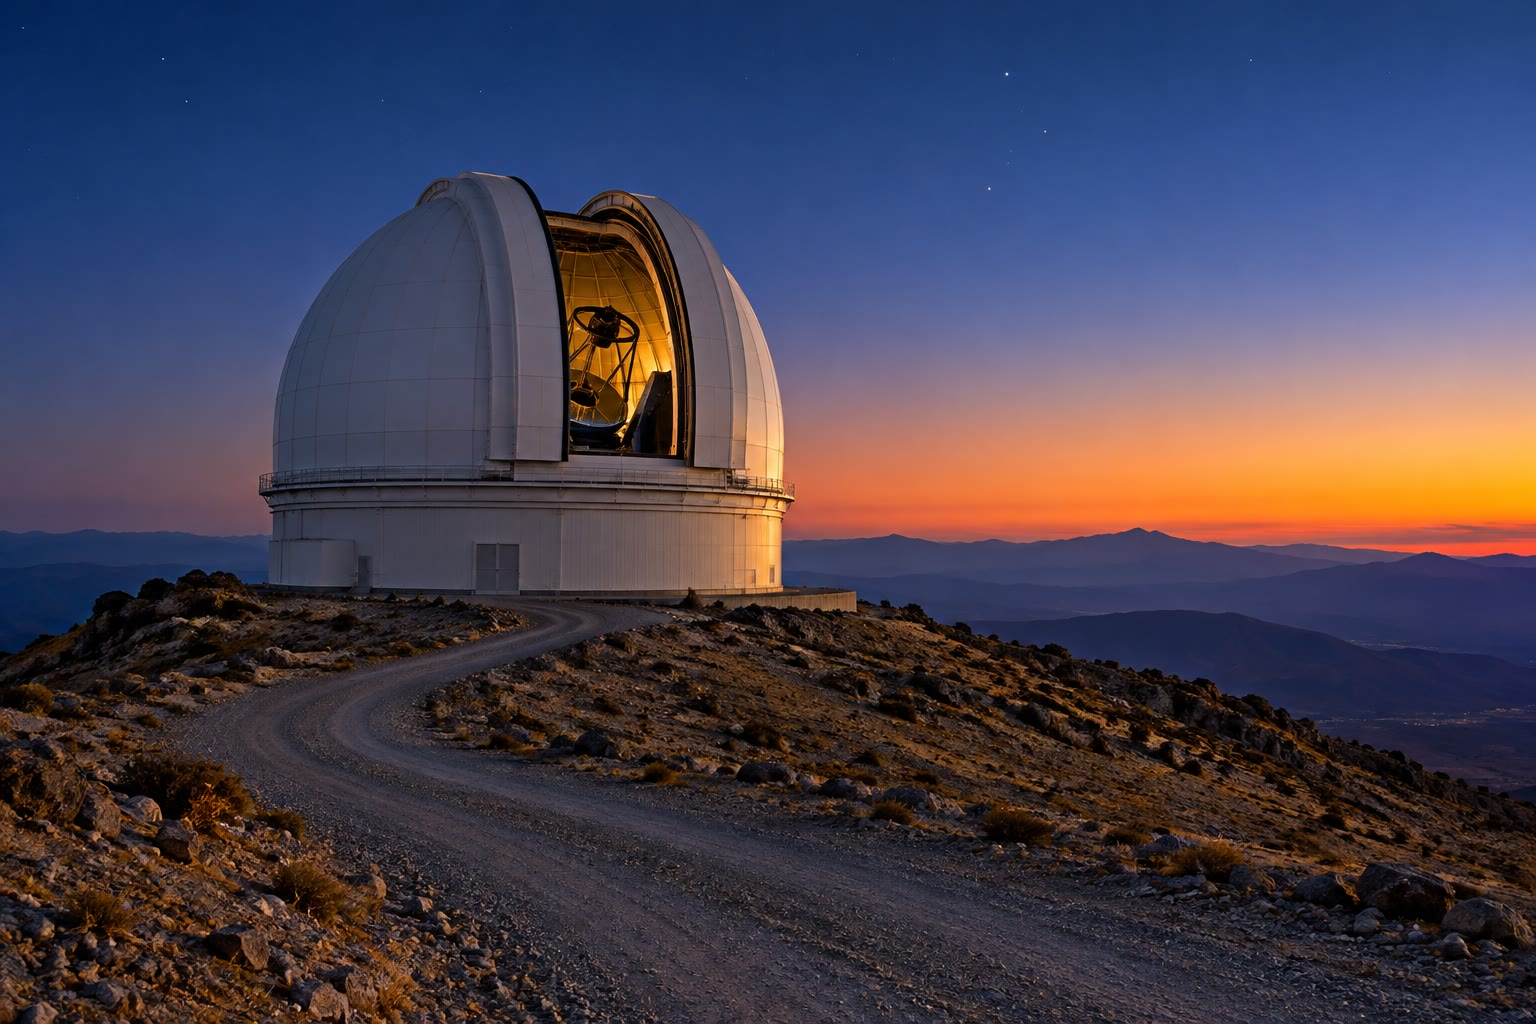
\includegraphics[width=0.55\linewidth]{images/book3/ai/b1-observatory-dusk.jpg}
\end{center}
\end{inthefield}

\section{Fluxos e magnitudes}\label{sec:b1:observing-the-sky:magnitudes}

\begin{definition}[Fluxo, luminosidade]\label{def:b1:observing-the-sky:flux}
O \emph{fluxo}\index{fluxo (de uma fonte)} $F$ recebido de uma fonte é a potência de sua radiação que atravessa uma área unitária mantida perpendicular à sua direção, em watts por metro quadrado; restrito a uma faixa de comprimentos de onda, é o fluxo nessa faixa. A \emph{luminosidade}\index{luminosidade} $L$ da fonte é a potência total que ela irradia, em watts.
\end{definition}

\begin{proposition}[Lei do inverso do quadrado]\label{prop:b1:observing-the-sky:inverse-square}
Uma fonte de \omterm{def:b1:observing-the-sky:flux}{luminosidade} $L$ que irradia igualmente em todas as direções, vista à distância $d$ através do espaço vazio, dá o \omterm{def:b1:observing-the-sky:flux}{fluxo}
\[
  F = \frac{L}{4\pi d^2} .
\]
\end{proposition}

\begin{proof}
Em regime estacionário, sem absorção, a potência que atravessa qualquer esfera centrada na fonte é a mesma, $L$, pela conservação da energia. Por simetria, ela se distribui uniformemente pela área da esfera, $4\pi d^2$.
\end{proof}

\begin{example}
A \omterm{def:b1:observing-the-sky:flux}{luminosidade} do Sol é \qty{3.828e26}{W}. A uma unidade astronômica,
\qty{1.496e11}{m}, seu \omterm{def:b1:observing-the-sky:flux}{fluxo} é $\num{3.828e26}/(4\pi\times
(\num{1.496e11})^2) = \qty{1361}{W.m^{-2}}$: a irradiância solar que a
Terra recebe no topo de sua atmosfera.
% ledger: sun:L, const:au, earth:TSI
\end{example}

Os \omterm{def:b1:observing-the-sky:flux}{fluxos} abrangem uma faixa enorme, e os astrônomos os comparam em uma escala logarítmica herdada das classes em que se separavam as estrelas visíveis a olho nu: as mais brilhantes de primeira magnitude, as mais fracas de sexta.

\begin{definition}[Magnitude aparente, banda fotométrica]\label{def:b1:observing-the-sky:magnitude}
Uma \emph{banda fotométrica}\index{banda fotométrica} é uma faixa de comprimentos de onda selecionada por um filtro padrão, designada por uma letra: U (ultravioleta), B (azul), V (visual), R (vermelho), I (infravermelho próximo), e J, H, K nas janelas do infravermelho.
A \emph{magnitude aparente}\index{magnitude aparente} $m$ de uma fonte em uma banda é definida a partir de seu \omterm{def:b1:observing-the-sky:flux}{fluxo} $F$ nessa banda por
\[
  m_1 - m_2 = -2.5\log_{10}\frac{F_1}{F_2} ,
\]
com o ponto zero fixado por estrelas padrão, próximo da magnitude da estrela Vega em cada banda. Uma diferença de 5 magnitudes corresponde a um fator exatamente igual a 100 no \omterm{def:b1:observing-the-sky:flux}{fluxo}; uma magnitude corresponde a um fator $100^{1/5} = 2.512$. Fontes mais brilhantes têm magnitudes menores, possivelmente negativas.
\end{definition}

Os comprimentos de onda centrais dos filtros padrão U, B, V, R e I são \qty{358.5}{nm}, \qty{437.1}{nm}, \qty{547.8}{nm}, \qty{650.4}{nm} e
\qty{802.0}{nm}.
% ledger: baldry:bessell-pivot
Na banda V, o Sol tem \omterm{def:b1:observing-the-sky:magnitude}{magnitude aparente} $-26.74$, Sirius, a estrela mais brilhante do céu noturno, $-1.46$, e Vega $0.03$. O Sol é, portanto, $10^{0.4\times(26.74 - 1.46)} = \num{1.29e10}$ vezes mais brilhante que Sirius em nosso céu; isso ainda não diz qual das duas brilha mais, para o que são necessárias as distâncias.
% ledger: nasa:sun-V, simbad:sirius, simbad:vega

\subsection*{Paralaxe e o parsec}

Enquanto a Terra gira em torno do Sol, uma estrela próxima parece deslocar-se contra o fundo de estrelas muito mais distantes, descrevendo em um ano uma pequena elipse. Esse movimento aparente é a medida mais direta das distâncias estelares: ele usa a órbita da Terra como base, como faz um agrimensor com a sua linha de base.

\begin{definition}[Paralaxe anual, parsec]\label{def:b1:observing-the-sky:parallax}
A \emph{paralaxe anual}\index{paralaxe anual} $p$ de uma estrela é o ângulo subentendido na estrela pelo raio da órbita da Terra, uma unidade astronômica, visto perpendicularmente à linha de visada; é o semieixo maior da elipse anual que a estrela parece descrever. O \emph{parsec}\index{parsec} (\unit{\parsec}) é a distância à qual uma unidade astronômica subtende um segundo de arco:
\[
  \qty{1}{\parsec} = \frac{\qty{1}{\au}}{\tan\ang{;;1}} = \qty{206265}{\au}
  = \qty{3.0857e16}{m} = \qty{3.2616}{\lightyear} .
\]
\end{definition}

Como $p$ é minúsculo, $\tan p \approx p$ em radianos, e a distância segue imediatamente:
\[
  d = \frac{\qty{1}{\au}}{\tan p} \quad\Longrightarrow\quad
  \frac{d}{\unit{\parsec}} = \frac{1}{p/\text{arcsec}} .
\]
Sirius tem paralaxe de \ang{;;0.37921}, logo está a $1/0.37921 =
\qty{2.637}{\parsec}$, \qty{8.60}{\lightyear}. Mesmo as estrelas mais próximas têm paralaxes inferiores a um segundo de arco, menores que o \omterm{def:b1:observing-the-sky:seeing}{seeing}: a paralaxe é obtida pelo deslocamento do centro da imagem da estrela, que muitos fótons localizam com precisão muito maior que a largura da imagem. Uma missão espacial descrita no fim deste capítulo mediu dessa forma as posições de quase dois bilhões de objetos.
% ledger: simbad:sirius, const:au, esa:gaia

\begin{omfigure}
\begin{tikzpicture}[font=\small]
\draw[black!50] (0,0) ellipse (2.0cm and 0.55cm);
\fill[orange!80!black] (0,0) circle (3pt) node[below=3pt] {Sol};
\fill[blue!70!black] (-2.0,0) circle (2pt) node[left, align=right] {Terra, seis\\ meses depois};
\fill[blue!70!black] (2.0,0) circle (2pt) node[right] {Terra};
\fill (0,4.4) circle (1.6pt) node[above] {estrela};
\draw[omDef, thick] (0,0) -- node[right, pos=0.55] {$d$} (0,4.4);
\draw[omThm] (2.0,0) -- (0,4.4);
\draw[omThm, dashed] (-2.0,0) -- (0,4.4);
\draw[thick] (0,0) -- node[above] {\qty{1}{\au}} (2.0,0);
\draw[omThm] (0,3.75) arc[start angle=-90, end angle=-65.6, radius=0.65cm];
\node[omThm] at (0.17,3.38) {$p$};
\end{tikzpicture}

{\small \omterm{def:b1:observing-the-sky:parallax}{Paralaxe anual} (fora de escala): vista da estrela, o raio da órbita da Terra subtende o ângulo $p$. Com seis meses de intervalo, a direção da estrela difere de $2p$. O ângulo real para a estrela mais próxima é inferior a um segundo de arco.}
\end{omfigure}

\begin{definition}[Magnitude absoluta, módulo de distância]\label{def:b1:observing-the-sky:absolute}
A \emph{magnitude absoluta}\index{magnitude absoluta} $M$ de uma estrela em uma banda é a \omterm{def:b1:observing-the-sky:magnitude}{magnitude aparente} que ela teria à distância de \qty{10}{\parsec}, vista através do espaço vazio. A diferença $m - M$ é o seu \emph{módulo de distância}\index{módulo de distância}.
\end{definition}

\begin{proposition}[O módulo de distância]\label{prop:b1:observing-the-sky:modulus}
Para uma estrela à distância $d$ vista através do espaço vazio,
\[
  m - M = 5\log_{10}\frac{d}{\qty{10}{\parsec}} .
\]
Se a luz é enfraquecida no caminho por $A$ magnitudes de extinção,
$m - M = 5\log_{10}(d/\qty{10}{\parsec}) + A$. Em uma banda, a razão entre as \omterm{def:b1:observing-the-sky:flux}{luminosidades} de duas estrelas é $L_1/L_2 = 10^{0.4(M_2 - M_1)}$.
\end{proposition}

\begin{proof}
Pela lei do inverso do quadrado, o \omterm{def:b1:observing-the-sky:flux}{fluxo} em $d$ e o \omterm{def:b1:observing-the-sky:flux}{fluxo} a \qty{10}{\parsec} estão na razão $F(d)/F(\qty{10}{\parsec}) = (\qty{10}{\parsec}/d)^2$. A definição de magnitudes dá $m - M = -2.5\log_{10}(\qty{10}{\parsec}/d)^2
= 5\log_{10}(d/\qty{10}{\parsec})$. A extinção multiplica o \omterm{def:b1:observing-the-sky:flux}{fluxo} por $10^{-0.4A}$, o que soma $A$ a $m$. À distância comum de \qty{10}{\parsec}, os \omterm{def:b1:observing-the-sky:flux}{fluxos} estão na razão das \omterm{def:b1:observing-the-sky:flux}{luminosidades}, e $M_1 - M_2 = -2.5\log_{10}(L_1/L_2)$.
\end{proof}

O Sol tem \omterm{def:b1:observing-the-sky:absolute}{magnitude absoluta} $M_\odot = 4.83$ e \omterm{def:b1:observing-the-sky:flux}{luminosidade} \qty{3.828e26}{W}. Comparando a \omterm{def:b1:observing-the-sky:absolute}{magnitude absoluta} de uma estrela na banda V com a do Sol, obtém-se a sua \omterm{def:b1:observing-the-sky:flux}{luminosidade} em V em unidades solares,
$L/L_\odot = 10^{0.4(4.83 - M)}$ --- uma \emph{\omterm{def:b1:observing-the-sky:flux}{luminosidade} na banda V}, já que uma estrela muito mais quente ou mais fria que o Sol coloca uma parte diferente de sua potência fora da banda V.
% ledger: sun:Mabs, sun:L

\subsection*{Cor}

\begin{definition}[Índice de cor]\label{def:b1:observing-the-sky:colour-index}
O \emph{índice de cor}\index{índice de cor} de uma estrela é a diferença de suas magnitudes em duas bandas, a mais azul primeiro; o mais usado é $B - V$. Um $B - V$ pequeno ou negativo marca uma estrela azul; um grande, uma estrela vermelha.
\end{definition}

O \omterm{def:b1:observing-the-sky:colour-index}{índice de cor} não depende da distância, pois a lei do inverso do quadrado reduz as duas bandas do mesmo modo; ele mede a forma do espectro e, portanto, a temperatura da superfície da estrela. Uma estrela irradia aproximadamente como um corpo negro cujo espectro tem pico em $\lambda_\mathrm{max} = b/T$ (lei de Wien, com
$b = \qty{2.898e-3}{m.K}$, recordada do volume de física do segundo ano).
A figura abaixo desenha três espectros de corpo negro: um corpo frio a \qty{3500}{K} tem pico no infravermelho próximo e dá mais \omterm{def:b1:observing-the-sky:flux}{fluxo} em V que em B; a temperatura efetiva do Sol, \qty{5772}{K}, põe seu pico em \qty{502}{nm}, entre B e V; um corpo a \qty{10000}{K} tem pico no ultravioleta e é mais brilhante em B que em V. A razão das radiâncias em B e V cresce de modo constante com a temperatura, de \num{0.46} a \num{0.97} e \num{1.53} para as três curvas, por isso $B - V$ diminui à medida que $T$ aumenta.
% ledger: const:b, nasa:sun-Teff, baldry:bessell-pivot

\begin{omfigure}
\begin{tikzpicture}
\begin{axis}[omrecord, width=0.9\linewidth, height=5.8cm, xmin=200, xmax=1500,
  ymin=0, ymax=1.17, xtick={200,400,...,1400}, ytick={0,0.5,1},
  xlabel={comprimento de onda (nm)},
  ylabel={$B_\lambda$ / máximo}, tick label style={font=\scriptsize},
  label style={font=\small}, legend style={font=\scriptsize, at={(0.5,1.03)},
  anchor=south, draw=none, fill=none}, legend columns=3]
\addplot[red!75!black, line width=1.1pt] table[x=lam_nm, y=t3500] {figdata/out/bachelor-1-blackbody_bands-curves.dat};
\addplot[orange!90!black, line width=1.1pt] table[x=lam_nm, y=t5772] {figdata/out/bachelor-1-blackbody_bands-curves.dat};
\addplot[omDef, line width=1.1pt] table[x=lam_nm, y=t10000] {figdata/out/bachelor-1-blackbody_bands-curves.dat};
\legend{\qty{3500}{K}, \qty{5772}{K} (o Sol), \qty{10000}{K}}
\draw[black!45, densely dashed] (axis cs:358.5,0) -- (axis cs:358.5,1.06);
\node[font=\scriptsize, above, inner sep=1pt] at (axis cs:358.5,1.06) {U};
\draw[black!45, densely dashed] (axis cs:437.1,0) -- (axis cs:437.1,1.06);
\node[font=\scriptsize, above, inner sep=1pt] at (axis cs:437.1,1.06) {B};
\draw[black!45, densely dashed] (axis cs:547.8,0) -- (axis cs:547.8,1.06);
\node[font=\scriptsize, above, inner sep=1pt] at (axis cs:547.8,1.06) {V};
\draw[black!45, densely dashed] (axis cs:650.4,0) -- (axis cs:650.4,1.06);
\node[font=\scriptsize, above, inner sep=1pt] at (axis cs:650.4,1.06) {R};
\draw[black!45, densely dashed] (axis cs:802.0,0) -- (axis cs:802.0,1.06);
\node[font=\scriptsize, above, inner sep=1pt] at (axis cs:802.0,1.06) {I};
\end{axis}
\end{tikzpicture}

{\small Espectros de corpo negro a três temperaturas, cada um dividido pelo seu próprio máximo, com os comprimentos de onda centrais dos filtros U, B, V, R e I (tracejados). O pico se desloca para comprimentos de onda menores à medida que a temperatura sobe (lei de Wien): \qty{828}{nm}, \qty{502}{nm} e \qty{290}{nm}.}
% ledger: const:h, const:c, const:kB, const:b, nasa:sun-Teff, baldry:bessell-pivot
\end{omfigure}

Quatro estrelas brilhantes mostram a faixa de cores:
\begin{center}
\small
\begin{tabular}{lcccc}
\hline
estrela & $V$ & $B$ & $B - V$ & paralaxe (\unit{mas}) \\
\hline
Rigel & 0.13 & 0.10 & $-0.03$ & 3.78 \\
Altair & 0.76 & 0.98 & 0.22 & 194.95 \\
Polaris & 2.02 & 2.62 & 0.60 & 7.54 \\
Betelgeuse & 0.42 & 2.27 & 1.85 & 6.55 \\
\hline
\end{tabular}
\end{center}
% ledger: simbad:rigel, simbad:altair, simbad:polaris, simbad:betelgeuse
Rigel é branco-azulada, e Betelgeuse, na mesma constelação, é laranja-avermelhada: uma diferença de cor visível a olho nu. Seus tipos espectrais, B8 e M1--M2, dizem o mesmo na linguagem dos espectros, assunto do Livro 5.

\section{Espectrógrafos}

A fotometria mede a luz em poucas bandas largas; um espectrógrafo a espalha em um espectro. A luz do foco do telescópio atravessa uma fenda estreita, é tornada paralela por um colimador, é dispersada por uma rede (ou por um prisma) e é focalizada por uma câmara sobre um detector, em que cada comprimento de onda cai em uma coluna diferente de pixels (veja a figura abaixo). Uma rede com $N$ linhas iluminadas, usada na ordem $k$, separa dois comprimentos de onda distantes de $\Delta\lambda$ quando $\lambda/\Delta\lambda \le kN$; esse é o seu poder de resolução (recordado do volume de física do segundo ano).

\begin{omfigure}
\begin{tikzpicture}[font=\scriptsize, >=Stealth]
\draw[thick, fill=omSea!25] (0.15,0) ellipse (0.13 and 0.9);
\node[below] at (0.15,-0.95) {objetiva};
\draw[omDef] (-1.3,0.75) -- (0.15,0.75) -- (2.4,0);
\draw[omDef] (-1.3,-0.75) -- (0.15,-0.75) -- (2.4,0);
\draw[omDef, ->] (-1.3,0) -- (-0.2,0);
\node[above] at (-0.8,0.75) {luz estelar};
\draw[very thick] (2.4,-0.35) -- (2.4,-0.06); \draw[very thick] (2.4,0.06) -- (2.4,0.35);
\node[above] at (2.4,0.38) {fenda};
\draw[omDef] (2.4,0) -- (3.6,0.55); \draw[omDef] (2.4,0) -- (3.6,-0.55);
\draw[thick, fill=omSea!25] (3.6,0) ellipse (0.1 and 0.72); \node[below] at (3.6,-0.74) {colimador};
\draw[omDef] (3.6,0.55) -- (4.9,0.55); \draw[omDef] (3.6,-0.55) -- (4.9,-0.55);
\draw[thick, pattern=north east lines] (4.85,-0.8) rectangle (5.0,0.8);
\node[below] at (4.92,-0.82) {rede};
\draw[blue!70!black] (5.0,0.3) -- (6.4,0.95); \draw[red!70!black] (5.0,0.3) -- (6.4,-0.15);
\draw[blue!70!black] (5.0,-0.3) -- (6.4,0.35); \draw[red!70!black] (5.0,-0.3) -- (6.4,-0.75);
\draw[thick, fill=omSea!25] (6.4,0.1) ellipse (0.1 and 1.08); \node[below] at (6.4,-1.0) {câmara};
\draw[blue!70!black] (6.4,0.95) -- (7.6,0.55); \draw[blue!70!black] (6.4,0.35) -- (7.6,0.55);
\draw[red!70!black] (6.4,-0.15) -- (7.6,-0.45); \draw[red!70!black] (6.4,-0.75) -- (7.6,-0.45);
\fill[black!70] (7.6,-0.8) rectangle (7.75,0.9);
\node[right, align=left] at (7.8,0.05) {detector:\\ um comprimento de onda\\ por coluna};
\end{tikzpicture}

{\small O percurso da luz por um telescópio e um espectrógrafo de rede (esquemático, com a objetiva do telescópio e a óptica desenhadas como lentes, e dois comprimentos de onda): a fenda isola a imagem da estrela, o colimador torna o feixe paralelo, a rede o dispersa, e a câmara focaliza cada comprimento de onda no seu próprio lugar no detector.}
\end{omfigure}

Um espectro traz três tipos de informação. Suas \emph{linhas}, escuras onde átomos e íons da atmosfera da estrela absorvem, e brilhantes onde um gás quente e rarefeito emite, identificam os elementos químicos presentes. A forma do contínuo e as intensidades relativas de linhas formadas em temperaturas diferentes dão a temperatura do gás. E o desvio Doppler das linhas dá a velocidade ao longo da linha de visada: uma linha de comprimento de onda de repouso $\lambda$ é deslocada de $\Delta\lambda = \lambda v_r/c$ para uma velocidade radial $v_r$ muito menor que $c$. Medir $v_r$ com \qty{1}{km.s^{-1}} exige um poder de resolução da ordem de $c/v_r = \num{300000}$, ou um poder de resolução moderado e muitas linhas medidas em conjunto. Como os espectros revelam a estrutura, a composição e os movimentos de estrelas e galáxias é o assunto do Livro 5.

\section{Observação a partir do espaço}

Acima da atmosfera não há bandas opacas, nem extinção, nem \omterm{def:b1:observing-the-sky:seeing}{seeing}, e no infravermelho nenhum brilho do ar aquecido. Os telescópios espaciais pagam por isso com custo, com a massa e o tamanho limitados que um foguete pode lançar e, na maioria deles, com a impossibilidade de reparo. São usados onde o solo não pode competir: para raios gama, raios X e ultravioleta, que nunca chegam ao solo; para o infravermelho além das janelas estreitas; para imagens no limite de difração sobre um campo amplo; e para medidas, como as paralaxes de um número muito grande de estrelas, que exigem um instrumento estável fora do ar turbulento.

\begin{dated}{2026}
% ledger: nasa:hubble-mirror, nasa:jwst-mirror, nasa:jwst-orbit, nasa:jwst-launch, nasa:jwst-range, esa:gaia
Três observatórios espaciais mostram a faixa. O Telescópio Espacial Hubble, lançado em 1990, tem um espelho primário de \qty{2.4}{m} de diâmetro. O Telescópio Espacial James Webb, lançado em 25 de dezembro de 2021, tem um espelho primário de \qty{6.5}{m} de diâmetro, formado por 18 segmentos hexagonais, com uma área coletora de \qty{25}{m^2}; ele opera de \qty{0.6}{\micro\metre} a \qty{28.5}{\micro\metre} e orbita o Sol perto do segundo ponto de Lagrange, L2, a \num{1.5}~milhão de quilômetros da Terra, do lado oposto ao Sol. O Gaia, lançado em 19 de dezembro de 2013 para a mesma região, usou dois telescópios com um plano focal comum de CCDs para mapear as posições e os movimentos de quase dois bilhões de objetos em três dimensões; suas observações estão concluídas, e seus catálogos estão sendo divulgados.
\end{dated}

\begin{omfigure}
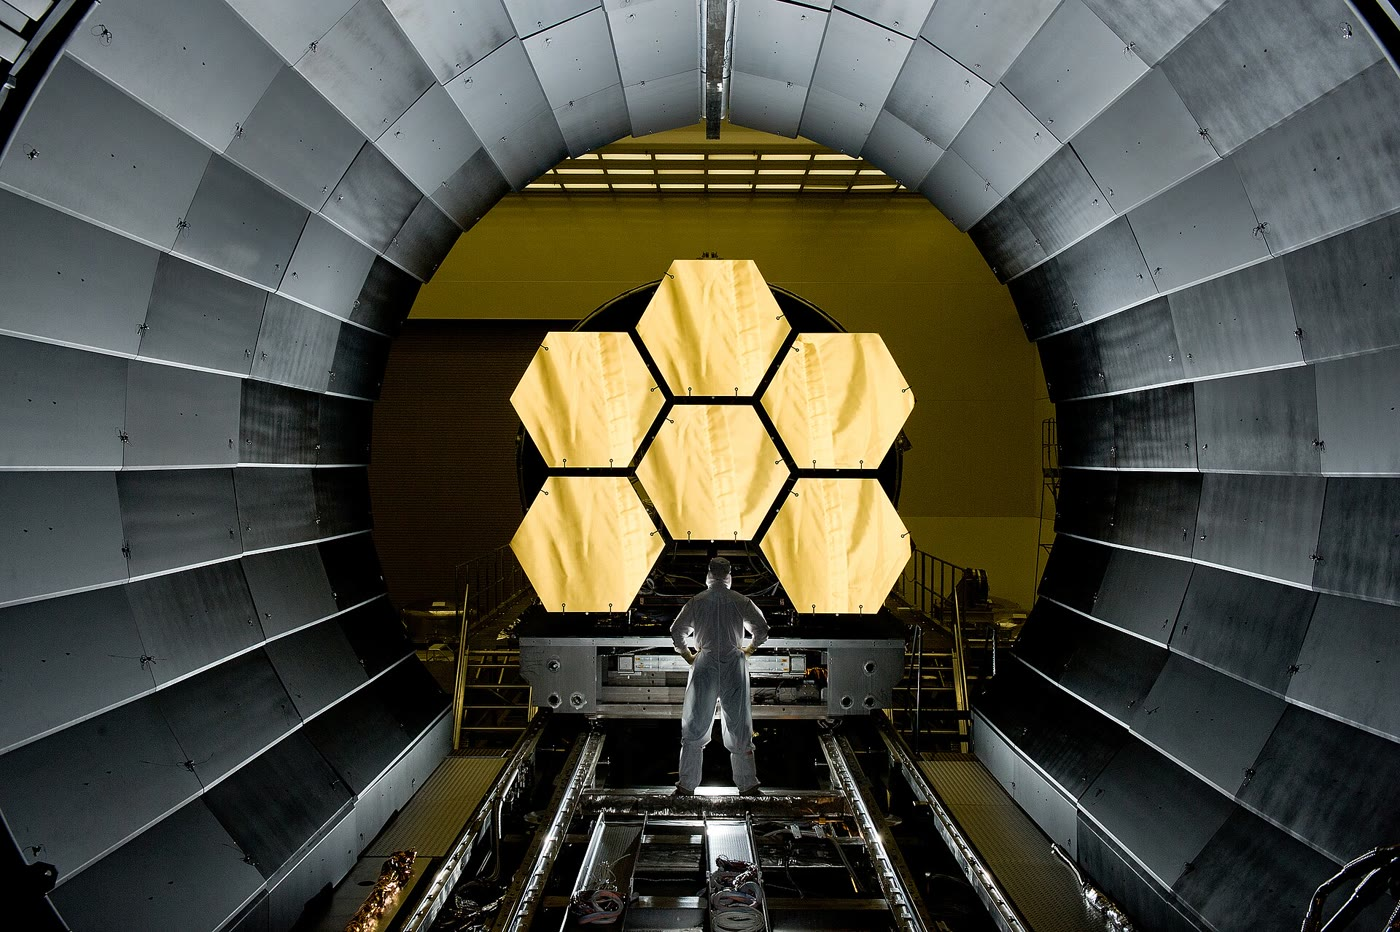
\includegraphics[width=0.78\linewidth]{images/book3/b1-jwst-mirror-segments.jpg}

{\small Seis dos 18 segmentos hexagonais do espelho primário do Telescópio Espacial James Webb, preparados para os testes em frio em 2011; juntos, desdobrados no espaço, os 18 formam um espelho de \qty{6.5}{m} de largura. Fotografia NASA/MSFC/David Higginbotham, domínio público.}
% ledger: commons:jwst-mirror, nasa:jwst-mirror
\end{omfigure}

\section{Exercícios}

\begin{exercise}[$\star$]\label{exo:b1:observing-the-sky:1}
Calcule a razão entre os \omterm{def:b1:observing-the-sky:flux}{fluxos} de duas estrelas de magnitudes 1.0 e 6.0, e a razão entre os de Rigel ($V = 0.13$) e Polaris ($V = 2.02$). Qual delas é mais brilhante no céu?
\end{exercise}

\begin{exercise}[$\star$]\label{exo:b1:observing-the-sky:2}
A paralaxe de Altair é \ang{;;0.19495}. Dê a sua distância em \omterm{def:b1:observing-the-sky:parallax}{parsecs}, em unidades astronômicas e em anos-luz.
\end{exercise}

\begin{exercise}[$\star$]\label{exo:b1:observing-the-sky:3}
Calcule o limite de difração de um telescópio espacial de \qty{2.4}{m} em \qty{550}{nm}, em segundos de arco, e compare-o com um \omterm{def:b1:observing-the-sky:seeing}{seeing} de \ang{;;0.40}. Faça o mesmo para um telescópio de \qty{6.5}{m} em \qty{2.0}{\micro\metre}.
\end{exercise}

\begin{exercise}[$\star$]\label{exo:b1:observing-the-sky:4}
A partir da tabela das quatro estrelas brilhantes, ordene Rigel, Altair, Polaris e Betelgeuse da superfície mais quente para a mais fria. Por que o \omterm{def:b1:observing-the-sky:colour-index}{índice de cor} pode ser comparado entre estrelas a distâncias muito diferentes?
\end{exercise}

\begin{exercise}[$\star\star$]\label{exo:b1:observing-the-sky:5}
Uma estrela é medida, na mesma noite, com magnitude 6.412 à distância zenital de \ang{30} e com 6.590 a \ang{60}. Admitindo uma atmosfera plano-paralela, calcule as duas \omterm{def:b1:observing-the-sky:extinction}{massas de ar}, o coeficiente de extinção e a magnitude da estrela acima da atmosfera.
\end{exercise}

\begin{exercise}[$\star\star$]\label{exo:b1:observing-the-sky:6}
Uma estrela dá 400 fotoelétrons numa exposição de \qty{10}{s}, e o ruído de fótons da própria estrela domina. Calcule a \omterm{def:b1:observing-the-sky:detector}{razão sinal-ruído}. Por quanto tempo é preciso expor para atingir uma SNR de 100? E para medir a magnitude com \num{0.01}?
\end{exercise}

\begin{exercise}[$\star\star$]\label{exo:b1:observing-the-sky:7}
Rigel tem $V = 0.13$ e paralaxe de \ang{;;0.00378}. Desprezando a extinção entre ela e nós, calcule sua distância, sua \omterm{def:b1:observing-the-sky:absolute}{magnitude absoluta} e sua \omterm{def:b1:observing-the-sky:flux}{luminosidade} na banda V em unidades solares ($M_\odot = 4.83$).
\end{exercise}

\begin{exercise}[$\star\star$]\label{exo:b1:observing-the-sky:8}
Compare as áreas coletoras de um espelho circular de \qty{2.4}{m} (ignore a sua obstrução central) e do telescópio Webb (\qty{25}{m^2}). Quantas vezes mais curta é a exposição em que o Webb coleta o mesmo número de fótons? Que fração de um disco cheio, de \qty{6.5}{m} de diâmetro, representa a sua área coletora, e por que essa fração é menor que um?
\end{exercise}

\begin{exercise}[$\star\star$]\label{exo:b1:observing-the-sky:9}
(a) A partir da \omterm{def:b1:observing-the-sky:flux}{luminosidade} do Sol, \qty{3.828e26}{W}, calcule o seu \omterm{def:b1:observing-the-sky:flux}{fluxo} a \qty{10}{\parsec}. (b) As \omterm{def:b1:observing-the-sky:magnitude}{magnitudes aparentes} e absoluta do Sol são $-26.74$ e $4.83$. Use o \omterm{def:b1:observing-the-sky:absolute}{módulo de distância} para recuperar a distância Sol--Terra, em unidades astronômicas.
\end{exercise}

\begin{exercise}[$\star\star\star$]\label{exo:b1:observing-the-sky:10}
Mostre, a partir de \cref{prop:b1:observing-the-sky:bouguer}, que $k =
2.5\log_{10}e\;\tau_0$. Para a noite da reta de extinção ($k =
\num{0.160}$), calcule a profundidade óptica no \omterm{def:b1:spherical-astronomy:celestial-sphere}{zênite} $\tau_0$ e a fração da luz que chega ao telescópio no \omterm{def:b1:spherical-astronomy:celestial-sphere}{zênite} e em $X = 2.31$. O que uma atmosfera plano-paralela preveria para a \omterm{def:b1:observing-the-sky:extinction}{massa de ar} a uma distância zenital de \ang{85}, e por que esse valor não deve ser confiável?
\end{exercise}

\begin{exercise}[$\star\star\star$]\label{exo:b1:observing-the-sky:11}
Uma galáxia fraca dá $R = 50$ fotoelétrons por segundo num telescópio, e o céu na área de sua imagem dá $B = \num{2000}$ por segundo quando o \omterm{def:b1:observing-the-sky:seeing}{seeing} é \ang{;;0.80}. O ruído de leitura é desprezível. (a) Por quanto tempo é preciso expor para uma SNR de 10? (b) O céu na imagem cresce com a área do disco de \omterm{def:b1:observing-the-sky:seeing}{seeing}. Repita para um \omterm{def:b1:observing-the-sky:seeing}{seeing} de \ang{;;0.40}. (c) Mostre que, para uma fonte muito mais fraca que o céu, o tempo de exposição necessário para uma dada SNR varia como $\theta^2/D^2$, em que $\theta$ é o \omterm{def:b1:observing-the-sky:seeing}{seeing} e $D$ o diâmetro do telescópio.
\end{exercise}

\begin{exercise}[$\star\star\star$]\label{exo:b1:observing-the-sky:12}
Uma rede com 1200 linhas por milímetro é iluminada em \qty{100}{mm} e usada na primeira ordem. (a) Qual é o seu poder de resolução, e qual é a menor diferença de comprimento de onda separável em \qty{550}{nm}? (b) A que velocidade radial corresponde essa diferença? (c) A Terra se move em torno do Sol a \qty{29.78}{km.s^{-1}}. Quanto esse movimento pode deslocar uma linha em \qty{550}{nm}, e quantos elementos de resolução isso representa? O que deve fazer, portanto, um observador que mede a velocidade de uma estrela?
% ledger: earth:vorb
\end{exercise}

\section{Problema: pesando a luz de Sirius}

\begin{problem}[{Problema de fim de semana --- quão longe está Sirius, quão brilhante ela parece, quantos fótons envia e quantos sóis ela ofusca}]
\label{pb:b1:observing-the-sky:1}
% ledger: simbad:sirius, simbad:vega, simbad:sirius-b, nasa:sun-V, sun:Mabs, const:au
% numbers computed in the scratch calculator calc/ch02.py from the rounded data
Sirius, a estrela mais brilhante do céu noturno, tem uma companheira fraca, a anã branca Sirius~B. Use os dados:
\begin{center}
\small
\begin{tabular}{lcc}
\hline
objeto & $V$ & paralaxe \\
\hline
Sirius & $-1.46$ & \ang{;;0.37921} \\
Sirius B & $8.44$ & --- \\
Vega & $0.03$ & \ang{;;0.13023} \\
o Sol & $-26.74$ & --- \\
\hline
\end{tabular}
\end{center}
com $M_\odot = 4.83$ na banda V, $\qty{1}{\parsec} = \qty{206265}{\au} =
\qty{3.0857e16}{m} = \qty{3.2616}{\lightyear}$, e um coeficiente de extinção $k = 0.15$ por \omterm{def:b1:observing-the-sky:extinction}{massa de ar} no observatório.

\medskip
\noindent\textbf{Parte I --- Quão longe está Sirius?}
\begin{enumerate}
  \item Calcule a distância de Sirius em \omterm{def:b1:observing-the-sky:parallax}{parsecs}.
  \item Exprima-a em unidades astronômicas e em metros.
  \item Exprima-a em anos-luz. Há quanto tempo a luz que vemos esta noite deixou Sirius?
  \item Ao longo de um ano, de que ângulo total a direção de Sirius oscila de um lado para o outro? Compare-o com um \omterm{def:b1:observing-the-sky:seeing}{seeing} de \ang{;;0.40}. Por que a oscilação ainda pode ser medida até uma pequena fração do \omterm{def:b1:observing-the-sky:seeing}{seeing}?
  \item Se a paralaxe estivesse errada em \ang{;;0.001}, de que fração a distância estaria errada, e de quantos anos-luz?
\end{enumerate}

\medskip
\noindent\textbf{Parte II --- Quão brilhante ela parece?}
\begin{enumerate}[resume]
  \item Calcule a razão entre os \omterm{def:b1:observing-the-sky:flux}{fluxos} de Sirius e de Vega na banda V.
  \item Calcule a razão entre os \omterm{def:b1:observing-the-sky:flux}{fluxos} do Sol e de Sirius.
  \item Calcule a razão entre os \omterm{def:b1:observing-the-sky:flux}{fluxos} de Sirius e de Sirius~B.
  \item Do Observatório do Paranal, Sirius cruza o meridiano a uma \omterm{def:b1:spherical-astronomy:horizontal}{altura angular} de \ang{82.09} (\cref{ch:b1:spherical-astronomy}). Calcule a \omterm{def:b1:observing-the-sky:extinction}{massa de ar}, a extinção e a magnitude medida naquele momento.
  \item Repita para uma \omterm{def:b1:spherical-astronomy:horizontal}{altura angular} de \ang{30}. Que fração da luz se perde no caminho?
  \item Por que a fórmula $X = \sec z$ induziria um observador em erro ao medir Sirius logo depois que ela nasce?
\end{enumerate}

\medskip
\noindent\textbf{Parte III --- Contando fótons.}
Uma câmera num telescópio de \qty{1}{m} registra $\num{3.0e4}$ fotoelétrons por segundo de uma estrela de magnitude $V = 10.0$, uma vez corrigida a extinção. Cada pixel contém no máximo $\num{1.0e5}$ elétrons (o seu poço cheio).
\begin{enumerate}[resume]
  \item Quantos fotoelétrons por segundo a câmera registra de Sirius~B?
  \item Qual é o tempo de exposição que dá a Sirius~B uma SNR de 1000, com o ruído de fótons da própria estrela? Qual é então o erro em sua magnitude?
  \item Quantos fotoelétrons por segundo a câmera registra de Sirius?
  \item Se \qty{20}{\percent} da luz de Sirius cai no seu pixel mais brilhante, quanto tempo esse pixel leva para se encher?
  \item Na imagem, as asas fracas da imagem de Sirius depositam, no lugar de Sirius~B, $10^{-4}$ da luz de Sirius por pixel, e o pixel mais brilhante de Sirius~B capta \qty{20}{\percent} da sua própria luz. Compare as duas taxas nesse pixel.
  \item Qual é a exposição mais longa que não satura esse pixel? Calcule a SNR de Sirius~B nesse pixel numa exposição de \qty{0.5}{s}, contando o ruído de fótons das duas fontes. Sirius~B é detectável, e o que a torna difícil?
\end{enumerate}

\medskip
\noindent\textbf{Parte IV --- Quantos sóis?}
\begin{enumerate}[resume]
  \item Calcule o \omterm{def:b1:observing-the-sky:absolute}{módulo de distância} de Sirius.
  \item Deduza a \omterm{def:b1:observing-the-sky:absolute}{magnitude absoluta} de Sirius na banda V, com duas casas decimais.
  \item Calcule a distância e a \omterm{def:b1:observing-the-sky:absolute}{magnitude absoluta} de Vega.
  \item Qual entre Sirius e Vega é intrinsecamente mais luminosa na banda V, e por que fator?
  \item Qual seria a \omterm{def:b1:observing-the-sky:magnitude}{magnitude aparente} do Sol vista à distância de Sirius? Tomando 6.0 como a magnitude mais fraca visível a olho nu numa noite escura, ela seria visível?
  \item Até que distância Sirius permaneceria visível a olho nu?
  \item Calcule a \omterm{def:b1:observing-the-sky:flux}{luminosidade} de Sirius na banda V em unidades solares: quantos sóis Sirius ofusca?
\end{enumerate}
\end{problem}
